% SOURCE: RG_gain_law_MERGED_REFIX20260730.json :: bundles.*.{gain_median_absdrop_per_dose,frac_drop_negative,family} (22 cells, family-coloured regimes)
% !TEX encoding = UTF-8 Unicode
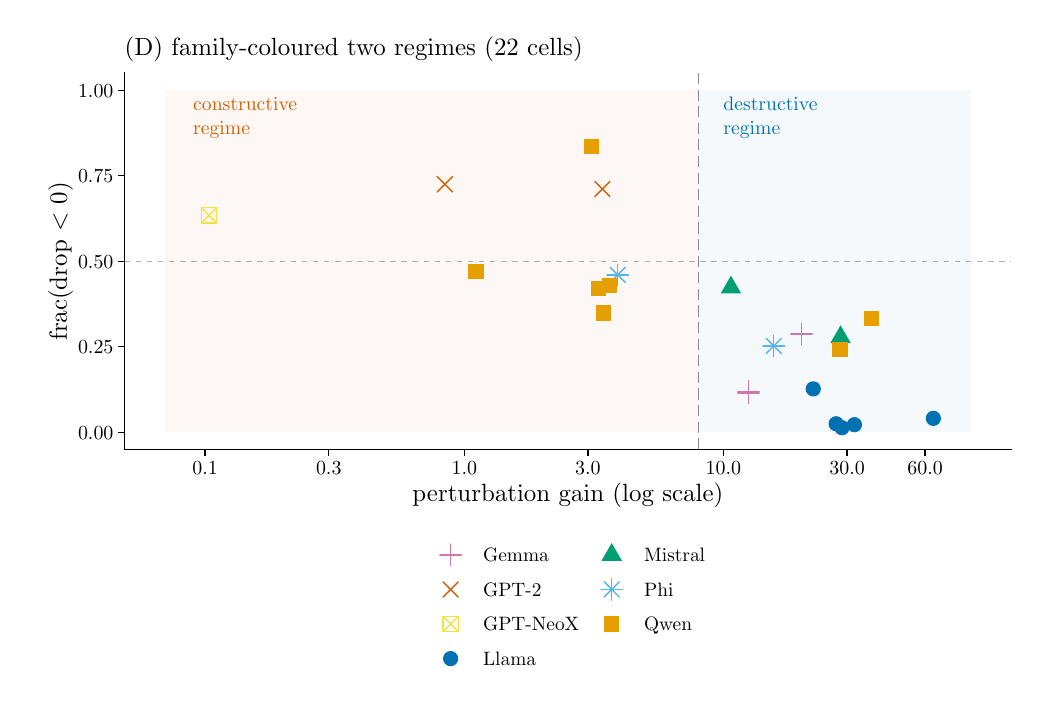
\begin{tikzpicture}[x=1pt,y=1pt]
\definecolor{fillColor}{RGB}{255,255,255}
\path[use as bounding box,fill=fillColor,fill opacity=0.00] (0,0) rectangle (361.35,238.49);
\begin{scope}
\path[clip] (  0.00,  0.00) rectangle (361.35,238.49);
\definecolor{drawColor}{RGB}{255,255,255}
\definecolor{fillColor}{RGB}{255,255,255}

\path[draw=drawColor,line width= 0.5pt,line join=round,line cap=round,fill=fillColor] (  0.00,  0.00) rectangle (361.35,238.49);
\end{scope}
\begin{scope}
\path[clip] ( 35.04, 86.11) rectangle (355.35,222.04);
\definecolor{fillColor}{RGB}{255,255,255}

\path[fill=fillColor] ( 35.04, 86.11) rectangle (355.35,222.04);
\definecolor{drawColor}{gray}{0.70}

\path[draw=drawColor,line width= 0.3pt,dash pattern=on 2pt off 2pt ,line join=round] ( 35.04,154.07) -- (355.35,154.07);
\definecolor{drawColor}{gray}{0.55}

\path[draw=drawColor,line width= 0.3pt,dash pattern=on 4pt off 2pt ,line join=round] (242.35, 86.11) -- (242.35,222.04);
\definecolor{fillColor}{RGB}{0,114,178}

\path[fill=fillColor,fill opacity=0.04] (242.35, 92.29) rectangle (340.79,215.86);
\definecolor{fillColor}{RGB}{213,94,0}

\path[fill=fillColor,fill opacity=0.04] ( 49.60, 92.29) rectangle (242.35,215.86);
\definecolor{drawColor}{RGB}{0,114,178}

\node[text=drawColor,anchor=base west,inner sep=0pt, outer sep=0pt, scale=  0.71] at (251.42,208.47) {destructive};

\node[text=drawColor,anchor=base west,inner sep=0pt, outer sep=0pt, scale=  0.71] at (251.42,199.82) {regime};
\definecolor{drawColor}{RGB}{213,94,0}

\node[text=drawColor,anchor=base west,inner sep=0pt, outer sep=0pt, scale=  0.71] at ( 59.83,208.47) {constructive};

\node[text=drawColor,anchor=base west,inner sep=0pt, outer sep=0pt, scale=  0.71] at ( 59.83,199.82) {regime};
\definecolor{fillColor}{RGB}{0,114,178}

\path[fill=fillColor] (283.87,107.97) circle (  2.75);

\path[fill=fillColor] (292.13, 95.37) circle (  2.75);

\path[fill=fillColor] (294.25, 93.93) circle (  2.75);

\path[fill=fillColor] (327.26, 97.32) circle (  2.75);

\path[fill=fillColor] (298.74, 95.02) circle (  2.75);
\definecolor{fillColor}{RGB}{0,158,115}

\path[fill=fillColor] (293.73,130.92) --
	(297.43,124.52) --
	(290.03,124.52) --
	cycle;

\path[fill=fillColor] (254.12,148.87) --
	(257.82,142.46) --
	(250.42,142.46) --
	cycle;
\definecolor{drawColor}{RGB}{86,180,233}

\path[draw=drawColor,line width= 0.5pt,line join=round,line cap=round] (266.85,120.73) -- (272.35,126.22);

\path[draw=drawColor,line width= 0.5pt,line join=round,line cap=round] (266.85,126.22) -- (272.35,120.73);

\path[draw=drawColor,line width= 0.5pt,line join=round,line cap=round] (265.72,123.48) -- (273.49,123.48);

\path[draw=drawColor,line width= 0.5pt,line join=round,line cap=round] (269.60,119.59) -- (269.60,127.36);

\path[draw=drawColor,line width= 0.5pt,line join=round,line cap=round] (210.48,146.38) -- (215.97,151.88);

\path[draw=drawColor,line width= 0.5pt,line join=round,line cap=round] (210.48,151.88) -- (215.97,146.38);

\path[draw=drawColor,line width= 0.5pt,line join=round,line cap=round] (209.34,149.13) -- (217.11,149.13);

\path[draw=drawColor,line width= 0.5pt,line join=round,line cap=round] (213.23,145.25) -- (213.23,153.02);
\definecolor{fillColor}{RGB}{230,159,0}

\path[fill=fillColor] (290.77,119.49) --
	(296.26,119.49) --
	(296.26,124.99) --
	(290.77,124.99) --
	cycle;

\path[fill=fillColor] (203.57,141.40) --
	(209.06,141.40) --
	(209.06,146.90) --
	(203.57,146.90) --
	cycle;

\path[fill=fillColor] (159.27,147.74) --
	(164.76,147.74) --
	(164.76,153.24) --
	(159.27,153.24) --
	cycle;

\path[fill=fillColor] (201.06,192.89) --
	(206.56,192.89) --
	(206.56,198.38) --
	(201.06,198.38) --
	cycle;

\path[fill=fillColor] (302.15,130.62) --
	(307.65,130.62) --
	(307.65,136.11) --
	(302.15,136.11) --
	cycle;

\path[fill=fillColor] (207.40,142.65) --
	(212.89,142.65) --
	(212.89,148.15) --
	(207.40,148.15) --
	cycle;

\path[fill=fillColor] (205.40,132.64) --
	(210.90,132.64) --
	(210.90,138.14) --
	(205.40,138.14) --
	cycle;
\definecolor{drawColor}{RGB}{204,121,167}

\path[draw=drawColor,line width= 0.5pt,line join=round,line cap=round] (275.76,127.80) -- (283.53,127.80);

\path[draw=drawColor,line width= 0.5pt,line join=round,line cap=round] (279.65,123.92) -- (279.65,131.69);

\path[draw=drawColor,line width= 0.5pt,line join=round,line cap=round] (256.56,106.46) -- (264.33,106.46);

\path[draw=drawColor,line width= 0.5pt,line join=round,line cap=round] (260.44,102.58) -- (260.44,110.34);

\path[draw=drawColor,line width= 0.5pt,line join=round,line cap=round] (256.58,106.99) -- (264.35,106.99);

\path[draw=drawColor,line width= 0.5pt,line join=round,line cap=round] (260.47,103.11) -- (260.47,110.88);
\definecolor{drawColor}{RGB}{240,228,66}

\path[draw=drawColor,line width= 0.5pt,line join=round,line cap=round] ( 62.76,167.94) rectangle ( 68.26,173.43);

\path[draw=drawColor,line width= 0.5pt,line join=round,line cap=round] ( 62.76,167.94) -- ( 68.26,173.43);

\path[draw=drawColor,line width= 0.5pt,line join=round,line cap=round] ( 62.76,173.43) -- ( 68.26,167.94);
\definecolor{drawColor}{RGB}{213,94,0}

\path[draw=drawColor,line width= 0.5pt,line join=round,line cap=round] (204.92,177.45) -- (210.41,182.95);

\path[draw=drawColor,line width= 0.5pt,line join=round,line cap=round] (204.92,182.95) -- (210.41,177.45);

\path[draw=drawColor,line width= 0.5pt,line join=round,line cap=round] (147.99,179.17) -- (153.48,184.66);

\path[draw=drawColor,line width= 0.5pt,line join=round,line cap=round] (147.99,184.66) -- (153.48,179.17);
\end{scope}
\begin{scope}
\path[clip] (  0.00,  0.00) rectangle (361.35,238.49);
\definecolor{drawColor}{RGB}{0,0,0}

\path[draw=drawColor,line width= 0.5pt,line join=round,line cap=rect] ( 35.04, 86.11) --
	( 35.04,222.04);
\end{scope}
\begin{scope}
\path[clip] (  0.00,  0.00) rectangle (361.35,238.49);
\definecolor{drawColor}{RGB}{0,0,0}

\node[text=drawColor,anchor=base east,inner sep=0pt, outer sep=0pt, scale=  0.72] at ( 30.99, 89.81) {0.00};

\node[text=drawColor,anchor=base east,inner sep=0pt, outer sep=0pt, scale=  0.72] at ( 30.99,120.70) {0.25};

\node[text=drawColor,anchor=base east,inner sep=0pt, outer sep=0pt, scale=  0.72] at ( 30.99,151.60) {0.50};

\node[text=drawColor,anchor=base east,inner sep=0pt, outer sep=0pt, scale=  0.72] at ( 30.99,182.49) {0.75};

\node[text=drawColor,anchor=base east,inner sep=0pt, outer sep=0pt, scale=  0.72] at ( 30.99,213.38) {1.00};
\end{scope}
\begin{scope}
\path[clip] (  0.00,  0.00) rectangle (361.35,238.49);
\definecolor{drawColor}{RGB}{0,0,0}

\path[draw=drawColor,line width= 0.5pt,line join=round] ( 32.79, 92.29) --
	( 35.04, 92.29);

\path[draw=drawColor,line width= 0.5pt,line join=round] ( 32.79,123.18) --
	( 35.04,123.18);

\path[draw=drawColor,line width= 0.5pt,line join=round] ( 32.79,154.07) --
	( 35.04,154.07);

\path[draw=drawColor,line width= 0.5pt,line join=round] ( 32.79,184.97) --
	( 35.04,184.97);

\path[draw=drawColor,line width= 0.5pt,line join=round] ( 32.79,215.86) --
	( 35.04,215.86);
\end{scope}
\begin{scope}
\path[clip] (  0.00,  0.00) rectangle (361.35,238.49);
\definecolor{drawColor}{RGB}{0,0,0}

\path[draw=drawColor,line width= 0.5pt,line join=round,line cap=rect] ( 35.04, 86.11) --
	(355.35, 86.11);
\end{scope}
\begin{scope}
\path[clip] (  0.00,  0.00) rectangle (361.35,238.49);
\definecolor{drawColor}{RGB}{0,0,0}

\path[draw=drawColor,line width= 0.5pt,line join=round] ( 64.11, 83.86) --
	( 64.11, 86.11);

\path[draw=drawColor,line width= 0.5pt,line join=round] (108.80, 83.86) --
	(108.80, 86.11);

\path[draw=drawColor,line width= 0.5pt,line join=round] (157.77, 83.86) --
	(157.77, 86.11);

\path[draw=drawColor,line width= 0.5pt,line join=round] (202.45, 83.86) --
	(202.45, 86.11);

\path[draw=drawColor,line width= 0.5pt,line join=round] (251.42, 83.86) --
	(251.42, 86.11);

\path[draw=drawColor,line width= 0.5pt,line join=round] (296.11, 83.86) --
	(296.11, 86.11);

\path[draw=drawColor,line width= 0.5pt,line join=round] (324.30, 83.86) --
	(324.30, 86.11);
\end{scope}
\begin{scope}
\path[clip] (  0.00,  0.00) rectangle (361.35,238.49);
\definecolor{drawColor}{RGB}{0,0,0}

\node[text=drawColor,anchor=base,inner sep=0pt, outer sep=0pt, scale=  0.72] at ( 64.11, 77.10) {0.1};

\node[text=drawColor,anchor=base,inner sep=0pt, outer sep=0pt, scale=  0.72] at (108.80, 77.10) {0.3};

\node[text=drawColor,anchor=base,inner sep=0pt, outer sep=0pt, scale=  0.72] at (157.77, 77.10) {1.0};

\node[text=drawColor,anchor=base,inner sep=0pt, outer sep=0pt, scale=  0.72] at (202.45, 77.10) {3.0};

\node[text=drawColor,anchor=base,inner sep=0pt, outer sep=0pt, scale=  0.72] at (251.42, 77.10) {10.0};

\node[text=drawColor,anchor=base,inner sep=0pt, outer sep=0pt, scale=  0.72] at (296.11, 77.10) {30.0};

\node[text=drawColor,anchor=base,inner sep=0pt, outer sep=0pt, scale=  0.72] at (324.30, 77.10) {60.0};
\end{scope}
\begin{scope}
\path[clip] (  0.00,  0.00) rectangle (361.35,238.49);
\definecolor{drawColor}{RGB}{0,0,0}

\node[text=drawColor,anchor=base,inner sep=0pt, outer sep=0pt, scale=  0.90] at (195.20, 67.25) {perturbation gain (log scale)};
\end{scope}
\begin{scope}
\path[clip] (  0.00,  0.00) rectangle (361.35,238.49);
\definecolor{drawColor}{RGB}{0,0,0}

\node[text=drawColor,rotate= 90.00,anchor=base,inner sep=0pt, outer sep=0pt, scale=  0.90] at ( 14.20,154.07) {frac(drop $<$ 0)};
\end{scope}
\begin{scope}
\path[clip] (  0.00,  0.00) rectangle (361.35,238.49);
\definecolor{fillColor}{RGB}{255,255,255}

\path[fill=fillColor] (141.11,  2.00) rectangle (249.29, 56.50);
\end{scope}
\begin{scope}
\path[clip] (  0.00,  0.00) rectangle (361.35,238.49);
\definecolor{fillColor}{RGB}{255,255,255}

\path[fill=fillColor] (145.61, 44.00) rectangle (160.06, 52.00);
\definecolor{drawColor}{RGB}{204,121,167}

\path[draw=drawColor,line width= 0.5pt,line join=round,line cap=round] (148.95, 48.00) -- (156.72, 48.00);

\path[draw=drawColor,line width= 0.5pt,line join=round,line cap=round] (152.83, 44.12) -- (152.83, 51.88);
\end{scope}
\begin{scope}
\path[clip] (  0.00,  0.00) rectangle (361.35,238.49);
\definecolor{fillColor}{RGB}{255,255,255}

\path[fill=fillColor] (145.61, 31.50) rectangle (160.06, 39.50);
\definecolor{drawColor}{RGB}{213,94,0}

\path[draw=drawColor,line width= 0.5pt,line join=round,line cap=round] (150.09, 32.75) -- (155.58, 38.25);

\path[draw=drawColor,line width= 0.5pt,line join=round,line cap=round] (150.09, 38.25) -- (155.58, 32.75);
\end{scope}
\begin{scope}
\path[clip] (  0.00,  0.00) rectangle (361.35,238.49);
\definecolor{fillColor}{RGB}{255,255,255}

\path[fill=fillColor] (145.61, 19.00) rectangle (160.06, 27.00);
\definecolor{drawColor}{RGB}{240,228,66}

\path[draw=drawColor,line width= 0.5pt,line join=round,line cap=round] (150.09, 20.25) rectangle (155.58, 25.75);

\path[draw=drawColor,line width= 0.5pt,line join=round,line cap=round] (150.09, 20.25) -- (155.58, 25.75);

\path[draw=drawColor,line width= 0.5pt,line join=round,line cap=round] (150.09, 25.75) -- (155.58, 20.25);
\end{scope}
\begin{scope}
\path[clip] (  0.00,  0.00) rectangle (361.35,238.49);
\definecolor{fillColor}{RGB}{255,255,255}

\path[fill=fillColor] (145.61,  6.50) rectangle (160.06, 14.50);
\definecolor{fillColor}{RGB}{0,114,178}

\path[fill=fillColor] (152.83, 10.50) circle (  2.75);
\end{scope}
\begin{scope}
\path[clip] (  0.00,  0.00) rectangle (361.35,238.49);
\definecolor{fillColor}{RGB}{255,255,255}

\path[fill=fillColor] (203.81, 44.00) rectangle (218.26, 52.00);
\definecolor{fillColor}{RGB}{0,158,115}

\path[fill=fillColor] (211.04, 52.27) --
	(214.74, 45.86) --
	(207.34, 45.86) --
	cycle;
\end{scope}
\begin{scope}
\path[clip] (  0.00,  0.00) rectangle (361.35,238.49);
\definecolor{fillColor}{RGB}{255,255,255}

\path[fill=fillColor] (203.81, 31.50) rectangle (218.26, 39.50);
\definecolor{drawColor}{RGB}{86,180,233}

\path[draw=drawColor,line width= 0.5pt,line join=round,line cap=round] (208.29, 32.75) -- (213.78, 38.25);

\path[draw=drawColor,line width= 0.5pt,line join=round,line cap=round] (208.29, 38.25) -- (213.78, 32.75);

\path[draw=drawColor,line width= 0.5pt,line join=round,line cap=round] (207.15, 35.50) -- (214.92, 35.50);

\path[draw=drawColor,line width= 0.5pt,line join=round,line cap=round] (211.04, 31.62) -- (211.04, 39.38);
\end{scope}
\begin{scope}
\path[clip] (  0.00,  0.00) rectangle (361.35,238.49);
\definecolor{fillColor}{RGB}{255,255,255}

\path[fill=fillColor] (203.81, 19.00) rectangle (218.26, 27.00);
\definecolor{fillColor}{RGB}{230,159,0}

\path[fill=fillColor] (208.29, 20.25) --
	(213.78, 20.25) --
	(213.78, 25.75) --
	(208.29, 25.75) --
	cycle;
\end{scope}
\begin{scope}
\path[clip] (  0.00,  0.00) rectangle (361.35,238.49);
\definecolor{drawColor}{RGB}{0,0,0}

\node[text=drawColor,anchor=base west,inner sep=0pt, outer sep=0pt, scale=  0.70] at (164.56, 45.59) {Gemma};
\end{scope}
\begin{scope}
\path[clip] (  0.00,  0.00) rectangle (361.35,238.49);
\definecolor{drawColor}{RGB}{0,0,0}

\node[text=drawColor,anchor=base west,inner sep=0pt, outer sep=0pt, scale=  0.70] at (164.56, 33.09) {GPT-2};
\end{scope}
\begin{scope}
\path[clip] (  0.00,  0.00) rectangle (361.35,238.49);
\definecolor{drawColor}{RGB}{0,0,0}

\node[text=drawColor,anchor=base west,inner sep=0pt, outer sep=0pt, scale=  0.70] at (164.56, 20.59) {GPT-NeoX};
\end{scope}
\begin{scope}
\path[clip] (  0.00,  0.00) rectangle (361.35,238.49);
\definecolor{drawColor}{RGB}{0,0,0}

\node[text=drawColor,anchor=base west,inner sep=0pt, outer sep=0pt, scale=  0.70] at (164.56,  8.09) {Llama};
\end{scope}
\begin{scope}
\path[clip] (  0.00,  0.00) rectangle (361.35,238.49);
\definecolor{drawColor}{RGB}{0,0,0}

\node[text=drawColor,anchor=base west,inner sep=0pt, outer sep=0pt, scale=  0.70] at (222.76, 45.59) {Mistral};
\end{scope}
\begin{scope}
\path[clip] (  0.00,  0.00) rectangle (361.35,238.49);
\definecolor{drawColor}{RGB}{0,0,0}

\node[text=drawColor,anchor=base west,inner sep=0pt, outer sep=0pt, scale=  0.70] at (222.76, 33.09) {Phi};
\end{scope}
\begin{scope}
\path[clip] (  0.00,  0.00) rectangle (361.35,238.49);
\definecolor{drawColor}{RGB}{0,0,0}

\node[text=drawColor,anchor=base west,inner sep=0pt, outer sep=0pt, scale=  0.70] at (222.76, 20.59) {Qwen};
\end{scope}
\begin{scope}
\path[clip] (  0.00,  0.00) rectangle (361.35,238.49);
\definecolor{drawColor}{RGB}{0,0,0}

\node[text=drawColor,anchor=base west,inner sep=0pt, outer sep=0pt, scale=  0.90] at ( 35.04,228.29) {(D) family-coloured two regimes (22 cells)};
\end{scope}
\end{tikzpicture}
